    \subsection{Docker Network Scheme}\label{subsec:ProjectNetworkScheme}
    \begin{center}
    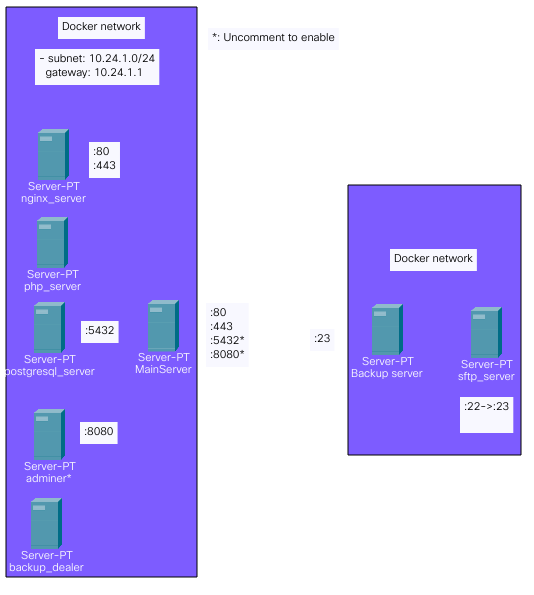
\includegraphics[scale=0.8]{NetworkDistribution}
    \end{center}
    \newpage

    \subsection{Docker Network Distribution Explanation}\label{subsec:dockernetworkdistribution-explanation}
    \begin{flushleft}
        As mentioned previously, the services are distributed in two servers, yet, the second one (the backup server),
        could be removed and store the backups locally, moving the \textbf{sftp} service to the main server, or, through
        \textbf{docker} using a volume or directory binding, but even if it's possible, it's recommended to do the backups in a
        different server as a security measure in case the main server get compromised.
    \end{flushleft}

    \begin{flushleft}
        Taking a look in the main server, we can see that the docker machines are mainly distributed among a common network,
        while there still an \textbf{docker} machine hanging by himself, that's because this \textbf{docker} machine is
        used to generate backups periodically, so doesn't need to have access to another docker networks (unless we wanted to specifically upload
        the backups inside a docker-machine that resides inside a docker network, but we didn't have the need
        to publish the ports in the main server, which is not the actual scenario, nor likely to happen).
    \end{flushleft}


    \subsubsection[Nginx]{Nginx}
    \begin{flushleft}
        Having the ports 80 and 443 exposed in the server, its configuration forces the use of the port 443, redirecting
        the connections fo that port, that way in case of having an HTTP petition the client is forced to use a "secure"
        connection, or at least, a connection that uses SSL encrypting.
    \end{flushleft}

    \subsubsection[PHP]{SFTP}
    \begin{flushleft}
        While this container doesn't do nothing by themself, either has ports exposed, it's linked to the nginx server, providing php support
        to that container.
    \end{flushleft}

    \subsubsection[Postgresql]{Postgresql}
    \begin{flushleft}
        PostgreSQL uses by default the port 5432 to connect to the databases, and while there could be some reasons to
        have it exposed, but since in this scenario we aren't making use of it, it's better to keep it closed, that way
        the connections are limited to the docker machines themselves.
    \end{flushleft}
    \newpage
    \subsubsection[Adminer]{Adminer}
    \begin{flushleft}
        Like previously mentioned, the ports from the database are not exposed, but, in case of needing a simple GUI
        access to them, this can be arranged by using the adminer docker, which provides a web-database management,
        and since it's in the same docker network than the postgresql database, we can have access to it without having
        to expose the ports.
        The active configuration allows you to access the service using the port 8080.
    \end{flushleft}

    \subsubsection[Portainer]{Portainer}
    \begin{flushleft}
        To provide easy access to monitor and control the docker volumes, have decided to implement \textbf{Portainer}
        to the docker network, allowing the users to access to it using the port 9000.
    \end{flushleft}


    \subsubsection[Backup\_dealer]{BackupDealer}
    \begin{flushleft}
       Like mentioned previously, this machine is used to periodically do backups of the desired volumes or directories,
       to a local volume or directory, or to a remote server.
       There isn't much to talk about it, since it doesn't provide a service by himself.
    \end{flushleft}

    \subsubsection[SFTP]{SFTP}
    \begin{flushleft}
        Observing the schema, we can see that the port 22 is being forwarded to the port 23, and publishing it, that's
        to avoid a port overlap with the default SSH port configuration.
    \end{flushleft}



    \newpage
    \subsection[Main Server Docker Configuration]{MainServerDockerConfiguration}\label{subsec:mainserverdockerconfiguration}
    \subsubsection[Main Server Docker-Compose]{Main Server DockerCompose}
    \lstinputlisting[language=Docker-compose,label={lst:MainDockerCompose}]{../docker-compose.yml}
    \paragraph{docker-compose.yml} that contains the services for the main server.
    \newpage
    \begin{flushleft}
        The main things worth to mention, besides the open ports which are already commented (yet again will be listed here),
        it's the restart policies and pointing out which services need to be build instead of using a raw image.
    \end{flushleft}
    \begin{enumerate}
        \item Networks:
            \begin{itemize}
                \item shop\_net:
                \begin{itemize}
                    \item nginx
                    \item php
                    \item adminer
                    \item postgresql
                \end{itemize}
                \item agent\_network:
                \begin{itemize}
                    \item portainer
                \end{itemize}
            \end{itemize}
        \item Volumes
            \begin{itemize}
                \item postgresql\_volume:
                \begin{itemize}
                      \item postgresql
                \end{itemize}
                \item portainer\_data:
                \begin{itemize}
                      \item portainer
                \end{itemize}
            \end{itemize}

    \end{enumerate}

    \begin{flushleft}
        All the dockers have been configured to restart in case of failure, which means that unless they are stopped manually,
        they will always restart.
    \end{flushleft}


    \newpage
    \subsubsection[PHP Dockerfile]{PHP Dockerfile}
    \lstinputlisting[language=Docker,label={lst:PHPDockerfile}]{../Dockerfiles/php}
    \begin{flushleft}
        As listed in the Dockerfile, it's main (and only) function, is to install and enable PDO extension for PHP\@.
    \end{flushleft}

    \newpage
    \subsubsection[Postgresql Dockerfile]{Postgresql Dockerfile}
    \lstinputlisting[language=Docker,label={lst:PostgresqlDockerfile}]{../Dockerfiles/postgresql/Dockerfile}
    \begin{flushleft}
        This Dockerfile, instead of installing new packages to the image, it adds a script that will be called in case
        of not having data in the postgres folder, and also adds an SQL files that once executed, will be deleted
        from the machine in order to avoid security flaws.
    \end{flushleft}

    \newpage
    \newpage
    \subsubsection[Backup Dealer Dockerfile]{Backup Dealer Dockerfile}
    \lstinputlisting[language=Docker,label={lst:BackupDealerlDockerfile}]{../Dockerfiles/backup_client/Dockerfile}
    \begin{flushleft}
        In comparison with the other 2 Dockerfiles which just fulfill one function, this one is more complex.
    \end{flushleft}
    \begin{flushleft}
        At the first Part it adds \textbf{Build} arguments and afterwards assign those arguments to environment variables
        to store its value in order to preserve it in future instances.

        Also initializes some variables with an empty value, which will require the user to specify them when using this docker.
    \end{flushleft}
    \begin{flushleft}
        Once the variables are set up, the Docker will install the packages required in order to accomplish its functions, which in this case the packages required are:
        \begin{itemize}
            \item : \textbf{Rsync} to generate backups from directories while keeping the permissions from the files.
            \item : \textbf{Tar} to compress the backups generated in order to reduce the size usage on the servers.
            \item : \textbf{Openssh} in order to be able to connect at the desired sftp server, so the backups can be
            item stored in a remote server.
            \item : \textbf{Keychain} so the backups can be fully automatized using certificates.
        \end{itemize}
    \end{flushleft}

    \begin{flushleft}
        Afterwards creates the default folders (based in the arguments given by the user, or using its default values),
        once it's done proceeds to add the file ".bashrc" with the content that will allow us to use a keychain avoiding the
        requirement of a password.
    \end{flushleft}
    \begin{flushleft}
        Finally, adds the "scripts" folder to the server.
    \end{flushleft}



